\documentclass[aspectratio=169]{beamer}

% Show speaker notes on second screen for pympress
\usepackage{pgfpages}
\setbeameroption{show notes on second screen=right}

% Match the existing CSE 534 Beamer styling
\usetheme{default}
\usecolortheme{default}
\setbeamertemplate{navigation symbols}{}
\setbeamertemplate{footline}[frame number]

\definecolor{darkbg}{HTML}{000000}
\definecolor{lighttext}{HTML}{999999}
\definecolor{miamired}{HTML}{941728}
\definecolor{codebg}{HTML}{1a1a1a}

\setbeamercolor{background canvas}{bg=darkbg}
\setbeamercolor{normal text}{fg=lighttext}
\setbeamercolor{frametitle}{fg=miamired}
\setbeamercolor{title}{fg=miamired}
\setbeamercolor{structure}{fg=miamired}
\setbeamercolor{item}{fg=miamired}
\setbeamercolor{block title}{fg=miamired,bg=codebg}
\setbeamercolor{block body}{fg=lighttext,bg=codebg}

\setbeamerfont{title}{series=\bfseries,size=\Large}
\setbeamerfont{frametitle}{series=\bfseries}

\usepackage{graphicx}
\usepackage{listings}
\usepackage{tikz}
\usepackage{array}
\usepackage{booktabs}
\usepackage{colortbl}
\usepackage{amsmath}
\usepackage{amssymb}
\usepackage{cancel}

\lstset{
    basicstyle=\ttfamily\small\color{lighttext},
    backgroundcolor=\color{codebg},
    keywordstyle=\color[HTML]{569cd6},
    commentstyle=\color[HTML]{6a9955},
    stringstyle=\color[HTML]{ce9178},
    showstringspaces=false,
    breaklines=true,
    frame=single,
    rulecolor=\color{codebg}
}

\setlength{\arrayrulewidth}{0.5pt}
\arrayrulecolor{miamired}
\renewcommand{\textbf}[1]{\textcolor{white}{\bfseries #1}}

\title{Normal Distributions and Linear Regression}
\subtitle{From discrete to continuous distributions}
\author{CSE 534}
\date{}

\begin{document}

\begin{frame}
\titlepage
\begin{center}
\textbf{Goal:} Model continuous values in generative AI
\end{center}
\note{Welcome to lesson 6. Today we're moving from discrete distributions to continuous ones. We'll explore the normal distribution and see how it connects to linear regression through maximum likelihood.}
\end{frame}

\begin{frame}[c]{Why continuous distributions?}
\textbf{So far:} Bernoulli or categorical distributions for discrete outcomes.

\vspace{0.5em}
\begin{itemize}
    \item Next-token prediction: pick from a vocabulary
    \item Classification: choose among fixed categories
\end{itemize}

\vspace{1em}
\textbf{But what about continuous values?}
\begin{itemize}
    \item An image is a 2D scalar field of pixel intensities
    \item Object positions are continuous coordinates
    \item Diffusion models move through continuous space
    \item Voice synthesis predicts continuous waveform amplitudes
\end{itemize}
\note{We've been working with discrete distributions---Bernoulli for binary outcomes, categorical for tokens or classes. But what about continuous values? A pixel intensity is a real number between 0 and 255, or normalized to 0 and 1. Object positions are x-y coordinates. Diffusion models move through continuous latent space. All of these require modeling real-valued outputs, not discrete bins.}
\end{frame}

\begin{frame}[c]{The normal distribution}
\textbf{One distribution appears repeatedly for continuous values:} the \emph{normal distribution}, also called the \emph{Gaussian}.

\vspace{1em}
\textbf{Why the Gaussian appears so often:}
\begin{itemize}
    \item Mathematically tractable---derivatives and integrals have closed forms
    \item Arises naturally when many small effects combine
    \item Maximum entropy distribution for a given mean and variance
    \item Captures correlations between continuous variables
\end{itemize}
\note{The Gaussian isn't universal, but it is widely applicable. Maximum entropy means that given only a mean and variance, the Gaussian makes the fewest additional assumptions. It doesn't impose hidden structure we don't know about. The correlation aspect---how pixel values or latent dimensions relate to each other---will become important when we extend to multivariate Gaussians in the next lesson.}
\end{frame}

\begin{frame}[c]{Historical context: Carl Friedrich Gauss}
\begin{columns}[c]
\begin{column}{0.65\textwidth}
\textbf{Early 1800s:} Gauss studied astronomical measurements.

\vspace{0.3em}
\textbf{The question:} When combining multiple measurements of the same quantity, which value is most likely to have produced those observations?

\vspace{0.5em}
\textbf{He already knew} the arithmetic mean worked well in practice.

\vspace{0.3em}
\textbf{He asked:} What error distribution would make the mean the maximum likelihood estimate?

\vspace{0.5em}
\textbf{Gauss's 1823 result:} The normal distribution is the \emph{only} one with this property.
\end{column}
\begin{column}{0.30\textwidth}
\centering
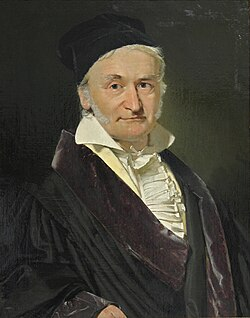
\includegraphics[width=\textwidth]{gauss_portrait.jpg}

\small Carl Friedrich Gauss (1777–1855)
\end{column}
\end{columns}
\note{People often think the normal distribution was just invented to fit data. But Gauss derived it from first principles by asking: what error distribution would make the arithmetic mean the maximum likelihood estimate? The normal distribution is the only one with this property. This is the same MLE reasoning we'll use today. Probabilistic thinking goes back centuries, long before modern statistics.}
\end{frame}

\begin{frame}[c]{The normal distribution formula}
\textbf{The normal density:}
\[
p(x; \mu, \sigma^2) = \frac{1}{\sqrt{2\pi\sigma^2}} \exp\left(-\frac{(x-\mu)^2}{2\sigma^2}\right)
\]

\vspace{0.5em}
\textbf{Parameters:}
\begin{itemize}
    \item $\mu$ (mu): the mean --- sets the center
    \item $\sigma^2$ (sigma squared): the variance --- controls the spread
    \item $\sigma$: the standard deviation
\end{itemize}

\vspace{0.5em}
\textbf{Interpretation:} Higher density values indicate regions where observations are more concentrated.
\note{Let's break down this formula. The exponential contains a squared term, (x minus mu)-squared. This penalizes deviations from mu---the farther x is from the center, the lower the probability density. The normalization constant in front, one over square-root of 2-pi-sigma-squared, ensures the total area under the curve is 1. Note that we square sigma in the formula, but we typically report sigma itself as the spread parameter. Variance is sigma-squared; standard deviation is sigma.}
\end{frame}

\begin{frame}[c]{Sampling from a normal distribution}
\begin{columns}[c]
\begin{column}{0.55\textwidth}
\textbf{Standard normal:} Sample $Z$ from a distribution with mean zero and variance one:
\[
Z \sim \mathcal{N}(0,1)
\]

\textbf{Transform to target:} Multiply by $\sigma$, add $\mu$:
\[
X = \mu + \sigma Z \sim \mathcal{N}(\mu, \sigma^2)
\]

\vspace{0.5em}
This scales the variance from 1 to $\sigma^2$ and shifts the mean from 0 to $\mu$.
\end{column}
\begin{column}{0.42\textwidth}
\centering
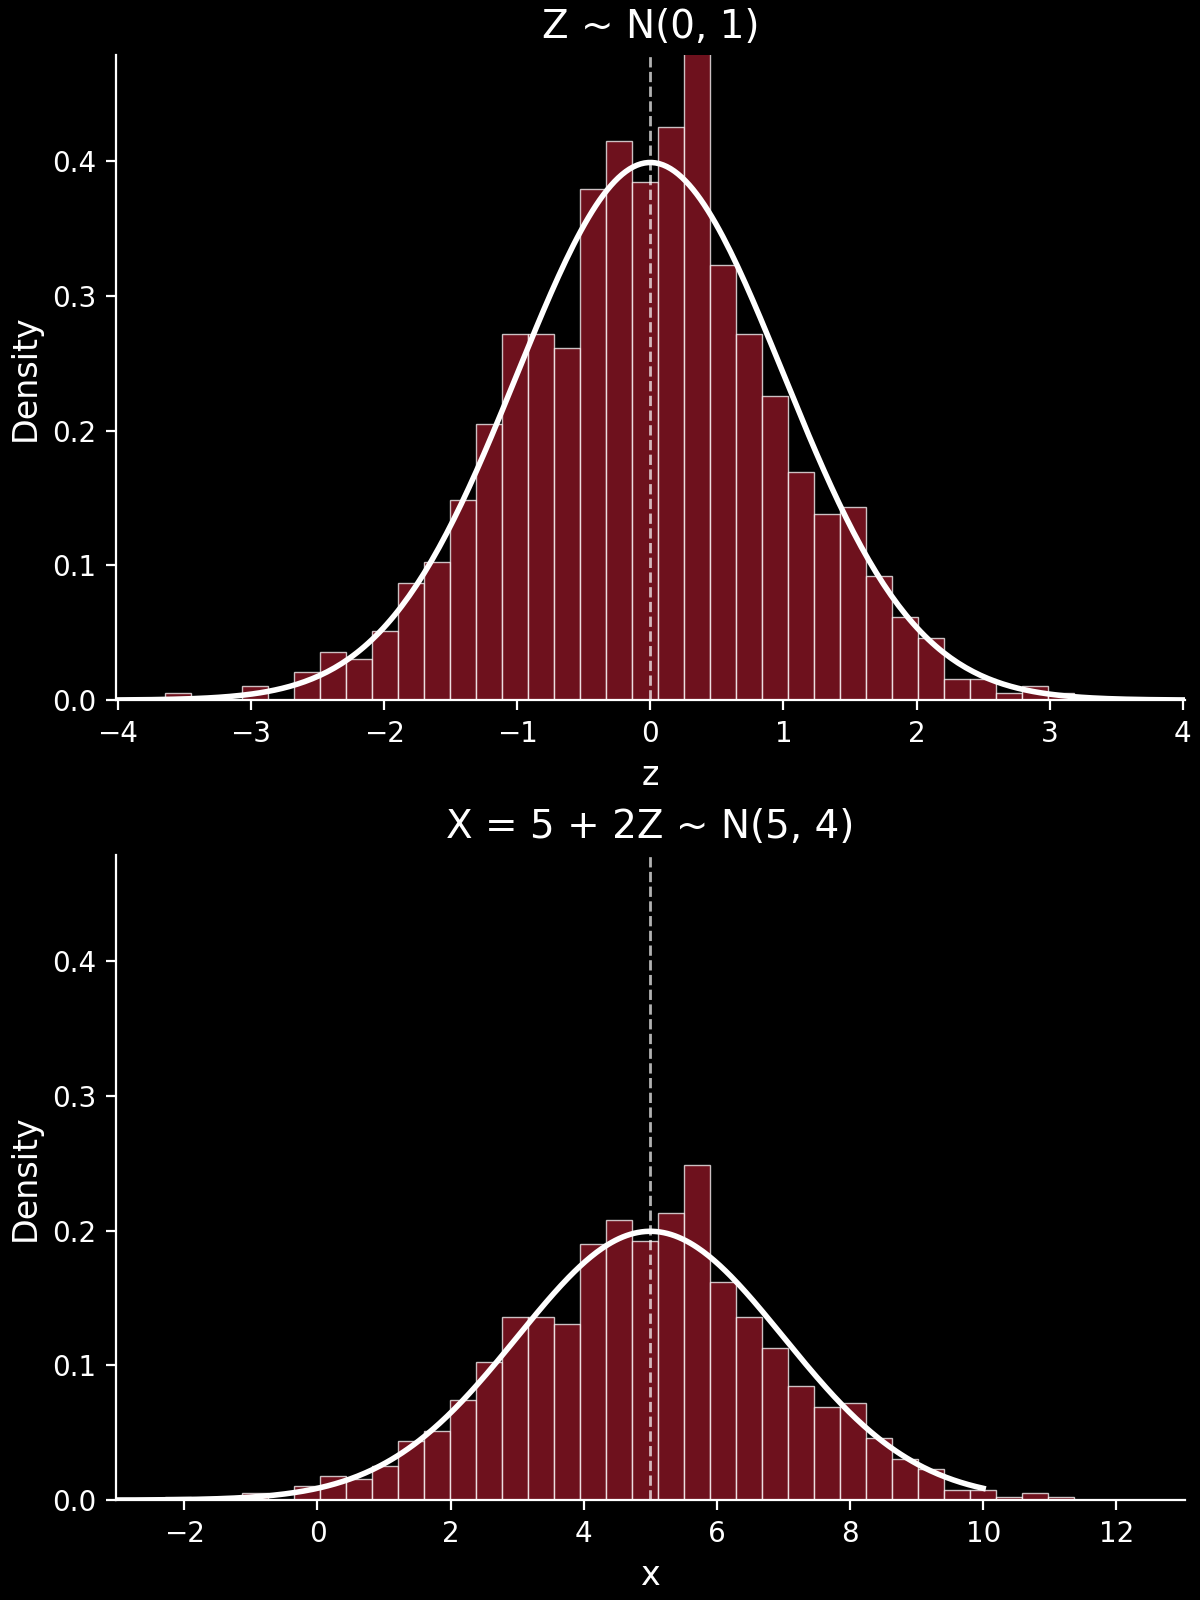
\includegraphics[width=\textwidth]{../08_normal/outputs/normal_shift_slides.png}
\end{column}
\end{columns}
\note{This is how sampling works in practice. NumPy gives you standard normal samples, mean zero and variance one. You transform them to match your target mean and variance. The tilde notation means "is distributed as" or "is sampled from." Order matters here: scale first by multiplying by sigma, then shift by adding mu. If you reverse this, you'll get the wrong variance. The figure shows Z from a standard normal on top, and X equals 5 plus 2Z, which gives us a normal with mean 5 and variance 4, on the bottom.}
\end{frame}

\begin{frame}[c]{The Central Limit Theorem}
\begin{columns}[c]
\begin{column}{0.48\textwidth}
\textbf{Central Limit Theorem:} The distribution of sample averages approaches normal as sample size grows.

\vspace{1em}
\textbf{Why it matters:} Even when individual observations aren't normal, their averages are approximately normal for large enough samples.

\vspace{1em}
\textbf{Example:} Draw 100 values from Uniform(0,1), compute their mean. Repeat 1000 times. The histogram of those means is approximately normal.
\end{column}
\begin{column}{0.48\textwidth}
\centering
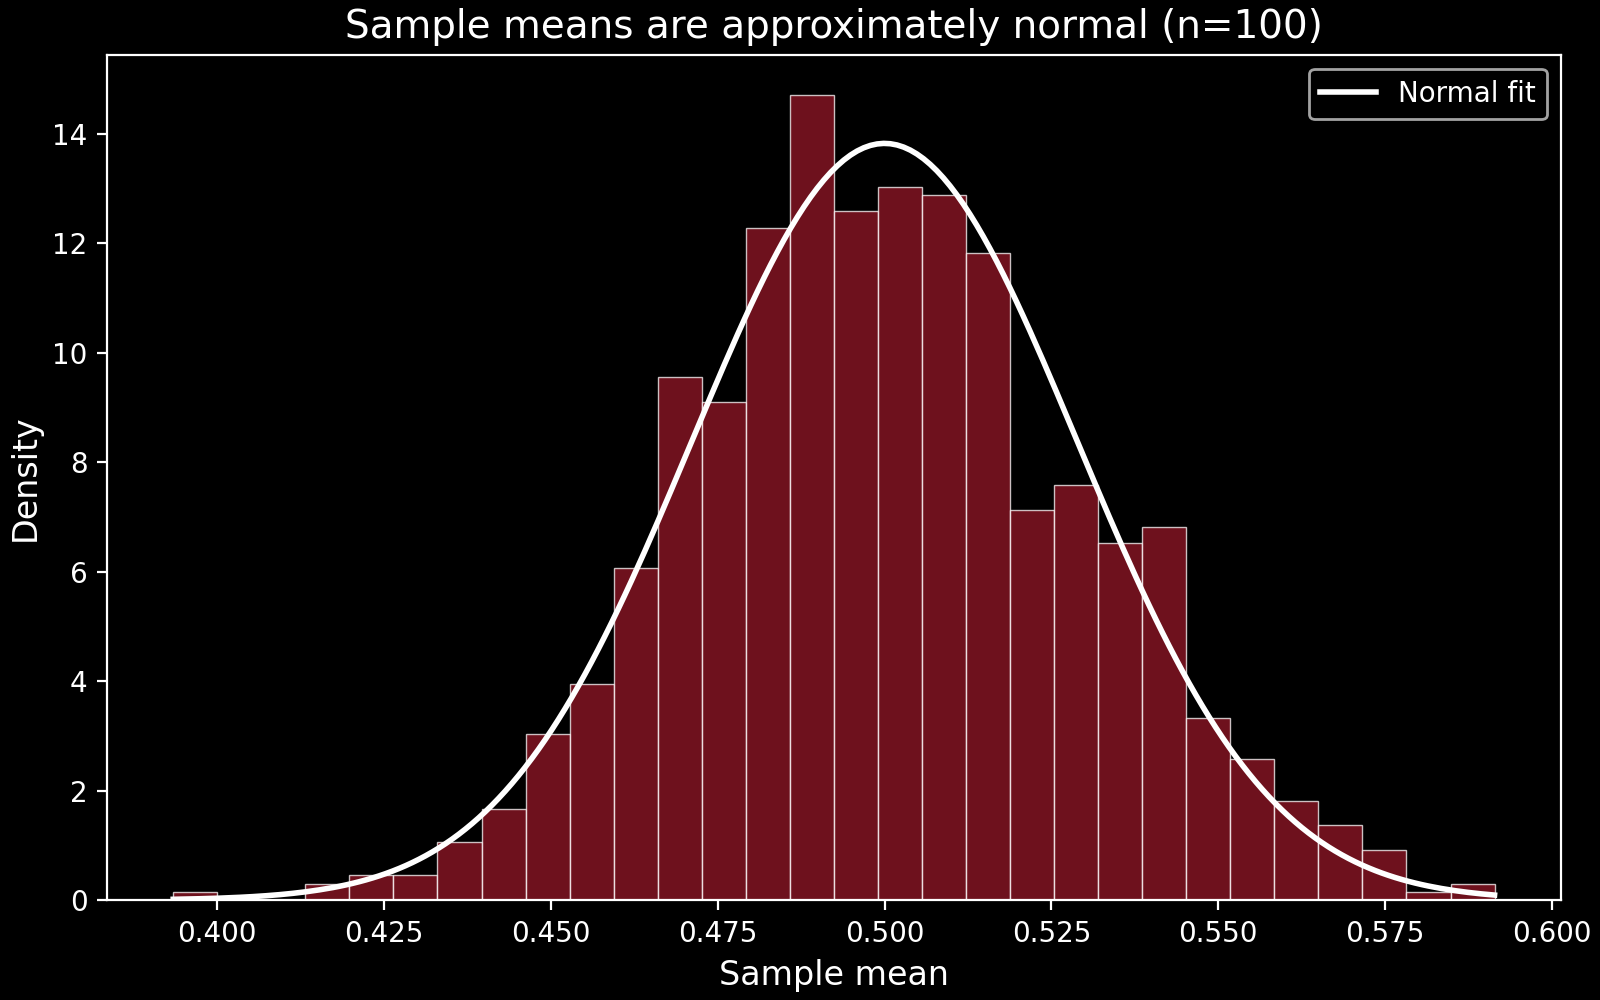
\includegraphics[width=\textwidth]{../08_normal/outputs/clt_demo.png}
\end{column}
\end{columns}
\note{The Central Limit Theorem is about distributions of averages, not individual observations. A common mistake is thinking "my data should be normal." No---the CLT says the mean of many samples is approximately normal, even if the individual samples aren't. This is why the normal distribution appears so often: many phenomena involve averages or sums of many small independent effects. The demo shows 1000 sample means, each computed from 100 uniform samples. The underlying distribution is flat, uniform, but the histogram of means is clearly normal.}
\end{frame}

\begin{frame}[c]{Maximum entropy property}
\textbf{Maximum entropy:} Among continuous distributions with fixed mean and variance, the normal has the greatest differential entropy.

\vspace{1em}
\textbf{What this means:} Given only the mean and variance, the Gaussian makes the fewest additional assumptions.

\vspace{1em}
\textbf{Why it matters:} When modeling uncertainty with limited information (mean and variance), the normal distribution is the least committal choice.

\vspace{1em}
\textbf{Connection to generative AI:} Variational autoencoders (VAEs) often use Gaussian priors in latent space precisely because of this maximum entropy property — it avoids introducing unjustified structure.
\note{Maximum entropy is subtle but important. It's not just about mathematical convenience---it's principled. If we know only the mean and variance, any distribution other than the Gaussian would impose additional structure beyond what we actually know. That's why Gaussian priors are so common in generative models. In VAEs, when we don't know the true latent distribution but want something tractable with controlled mean and variance, the Gaussian is the natural, least-committal choice.}
\end{frame}

\begin{frame}[c]{Maximum likelihood for the mean}
\textbf{Suppose} you observe $x_1, x_2, \ldots, x_n$ drawn independently from a normal distribution.

\vspace{0.5em}
\textbf{Question:} Which values of $\mu$ and $\sigma^2$ make the observed data most probable?

\vspace{1em}
\textbf{The sample mean} is the maximum likelihood estimate for $\mu$:
\[
\hat{\mu}_{\text{MLE}} = \frac{1}{n} \sum_i x_i
\]

\vspace{0.5em}
This connects to Gauss's original insight: the normal distribution justifies the arithmetic mean as the optimal estimate.
\note{We'll derive this in the next slides. The key insight is that the likelihood function tells us how probable our data is for different parameter values. By maximizing it, we find the parameter that makes our observed data most likely.}
\end{frame}

\begin{frame}[c]{Derivation: Start with the Gaussian}
\textbf{Single observation:} The probability density is
\[
p(x \mid \mu, \sigma^2) = \frac{1}{\sqrt{2\pi\sigma^2}} \exp\left(-\frac{(x - \mu)^2}{2\sigma^2}\right)
\]

\vspace{1em}
\textbf{Independent observations:} Multiply the densities
\[
p(x_1, \ldots, x_n \mid \mu, \sigma^2) = \prod_{i=1}^n \frac{1}{\sqrt{2\pi\sigma^2}} \exp\left(-\frac{(x_i - \mu)^2}{2\sigma^2}\right)
\]

\vspace{1em}
\textbf{This is the likelihood function} $\mathcal{L}(\mu, \sigma^2)$ we want to maximize.
\note{Independence is key---it lets us multiply the individual probabilities. The product of exponentials will become a sum when we take the log, which is why log-likelihood is easier to work with. Remember that we're treating the data as fixed and the parameters as variables.}
\end{frame}

\begin{frame}[c]{Derivation: Negative log-likelihood (ignore constants)}
\textbf{Take the log:}
\[
\log \mathcal{L} = \sum_{i=1}^n \left[-\frac{1}{2}\log(2\pi\sigma^2) - \frac{(x_i - \mu)^2}{2\sigma^2}\right]
\]

\vspace{1em}
\textbf{Negate and drop constants that don't depend on $\mu$:}
\[
\text{NLL}(\mu) = \frac{1}{2\sigma^2} \sum_{i=1}^n (x_i - \mu)^2
\]

\vspace{1em}
\textbf{Goal:} Minimize this with respect to $\mu$.
\note{We dropped the log(2pi*sigma-squared) term because it doesn't contain mu, so it doesn't affect where the minimum occurs. We're also treating sigma-squared as a constant here since we're only optimizing for mu. The sum of squared deviations should look familiar---it's the same objective we'd get from least squares.}
\end{frame}

\begin{frame}[c]{Derivation: Take the derivative}
\textbf{Differentiate NLL with respect to $\mu$:}
\[
\frac{\partial}{\partial \mu} \left[\frac{1}{2\sigma^2} \sum_{i=1}^n (x_i - \mu)^2\right]
\]

\vspace{1em}
\textbf{Apply the chain rule:}
\[
= \frac{1}{2\sigma^2} \sum_{i=1}^n 2(x_i - \mu) \cdot (-1)
\]

\vspace{1em}
\textbf{Simplify:}
\[
= -\frac{1}{\sigma^2} \sum_{i=1}^n (x_i - \mu)
\]
\note{The 2 from the chain rule cancels with the 1/2 in front. The derivative of (xi - mu)-squared is 2(xi - mu), and the derivative of -mu with respect to mu is -1. Sign errors are common here, so double-check each step.}
\end{frame}

\begin{frame}[c]{Derivation: Solve for $\mu$}
\textbf{Set the derivative to zero:}
\[
-\frac{1}{\sigma^2} \sum_{i=1}^n (x_i - \mu) = 0
\]

\vspace{1em}
\textbf{Multiply both sides by $-\sigma^2$:}
\[
\sum_{i=1}^n (x_i - \mu) = 0
\]

\vspace{1em}
\textbf{Expand:}
\[
\sum_{i=1}^n x_i - n\mu = 0
\]

\vspace{1em}
\textbf{Solve for $\mu$:}
\[
\hat{\mu}_{\text{MLE}} = \frac{1}{n} \sum_{i=1}^n x_i
\]

\vspace{0.5em}
The maximum likelihood estimate is the sample mean.
\note{This is a minimum of NLL, which is a maximum of the likelihood. You can verify it's a minimum by checking the second derivative is positive. This derivation shows why the arithmetic mean is the right thing to compute---it falls out of the math when we assume a Gaussian model.}
\end{frame}

\begin{frame}[c]{Maximum likelihood for the variance}
\textbf{Similarly,} we can find the MLE for $\sigma^2$.

\vspace{1em}
\textbf{The sample variance} that maximizes likelihood:
\[
\hat{\sigma}^2_{\text{MLE}} = \frac{1}{n} \sum_i (x_i - \hat{\mu}_{\text{MLE}})^2
\]

\vspace{1em}
\textbf{Problem:} This estimate is \emph{biased} --- it systematically underestimates the true variance.

\vspace{1em}
\textbf{Expected value:}
\[
\mathbb{E}\left[\hat{\sigma}^2_{\text{MLE}}\right] = \frac{n-1}{n}\sigma^2 \neq \sigma^2
\]
\note{The derivation follows the same log-likelihood pattern we used for mu: take the derivative with respect to sigma-squared, set to zero, and solve. The key result: MLE gives the average squared deviation from the sample mean. This is straightforward to compute, but MLE does not guarantee unbiasedness. The expectation formula shows the bias factor is (n-1)/n. For large n, is this a big problem? No, but for small samples the bias matters---with n=5, we underestimate by 20 percent.}
\end{frame}

\begin{frame}[c]{Why is the MLE biased?}
\textbf{Key insight:} Variance around the true mean $\mu$ has two components.

\vspace{0.5em}
\textbf{Variance decomposition:} \quad $\displaystyle \text{Var}(X - \mu) = \text{Var}(X - \hat{\mu}) + \text{Var}(\hat{\mu})$

\vspace{0.2em}
{\tiny (The cross terms cancel because $\mathbb{E}[X - \hat{\mu}] = 0$)}

\pause
\vspace{0.5em}

\textbf{In other words:}
\begin{align*}
\sigma^2 &= \mathbb{E}[(X - \hat{\mu})^2] + \text{Var}(\hat{\mu})\\[0.3em]
&= \mathbb{E}[(X - \hat{\mu})^2] + \frac{\sigma^2}{n}
\end{align*}

\pause
\vspace{0.5em}

\textbf{Subtract $\sigma^2/n$ from both sides:} \quad $\displaystyle \sigma^2 - \frac{\sigma^2}{n} = \mathbb{E}[(X - \hat{\mu})^2]$

\pause
\vspace{0.5em}

\textbf{What we measure:} $\frac{1}{n}\sum_i (x_i - \hat{\mu})^2$ estimates $\mathbb{E}[(X - \hat{\mu})^2]$

\textbf{What we're missing:} The variance of the sample mean, $\sigma^2/n$
\note{This is the crucial point: total variance = variance around sample mean + variance of sample mean. The decomposition works because when you expand (X - mu)² = ((X - mu-hat) + (mu-hat - mu))² and take expectations, the cross term 2E[(X - mu-hat)(mu-hat - mu)] = 2(mu-hat - mu)E[X - mu-hat] = 0, since by definition the deviations from the sample mean average to zero.

[click]

The sample mean itself is a random variable with variance sigma²/n. When we compute deviations from the sample mean instead of the true mean, we're ignoring this component.

[click]

The algebra: sigma² = E[(X - mu-hat)²] + sigma²/n, so E[(X - mu-hat)²] = sigma²(1 - 1/n) = sigma²(n-1)/n.

[click]

We measure (1/n) times the sum of (xi - mu-hat)², which estimates E[(X - mu-hat)²], but we're missing the variance of the sample mean, sigma²/n.}
\end{frame}

\begin{frame}[c]{Bessel's correction}
\begin{align*}
\onslide<1->{\text{\textbf{Starting from the previous slide:}} \quad
\sigma^2 - \frac{\sigma^2}{n} &= \mathbb{E}[(X - \hat{\mu})^2]\\[0.5em]}
\onslide<2->{\text{\textbf{Factor out $\sigma^2$:}} \quad
\sigma^2\left(1 - \frac{1}{n}\right) &= \mathbb{E}[(X - \hat{\mu})^2]\\[0.5em]}
\onslide<3->{\text{\textbf{Common denominator:}} \quad
\sigma^2 \frac{n-1}{n} &= \mathbb{E}[(X - \hat{\mu})^2]\\[0.5em]}
\onslide<4->{\text{\textbf{Multiply by $\frac{n}{n-1}$:}} \quad
\sigma^2 &= \frac{n}{n-1}\mathbb{E}\left[(X - \hat{\mu})^2\right]\\[0.5em]}
\onslide<5->{\text{\textbf{Sample estimate:}} \quad
\sigma^2 &\approx \frac{\cancel{n}}{n-1} \cdot \frac{1}{\cancel{n}}\sum_i(x_i - \hat{\mu})^2\\[0.5em]}
\onslide<6->{&= \frac{1}{n-1}\sum_i(x_i - \hat{\mu})^2}
\end{align*}
\note{Starting from the previous slide: sigma² minus sigma²/n equals the expected value of (X - mu-hat)².

[click]

Factor out sigma²: sigma²(1 - 1/n) equals E[(X - mu-hat)²].

[click]

Common denominator: sigma² times (n-1)/n equals E[(X - mu-hat)²].

[click]

Multiply both sides by n/(n-1): sigma² equals (n/(n-1)) times E[(X - mu-hat)²].

[click]

For the sample estimate: sigma² is approximately (n/(n-1)) times (1/n) times the sum of (xi - mu-hat)².

[click]

Cancel the n's: the n in the numerator cancels with the n in the denominator, leaving 1/(n-1) times the sum. This is Bessel's correction---divide by n-1 instead of n. Most software (R, pandas) uses n-1 by default. NumPy's var() has ddof=0 (biased) by default, but use ddof=1 for unbiased.}
\end{frame}

\begin{frame}[c]{The unbiased estimator}
\textbf{Result:}
\[
\hat{\sigma}^2_{\text{unbiased}} = \frac{1}{n-1} \sum_i (x_i - \hat{\mu})^2
\]

\vspace{1em}
\textbf{Summary:}
\begin{itemize}
    \item MLE gives $\frac{1}{n}\sum_i(x_i - \hat{\mu})^2$ (biased)
    \item Unbiased estimator uses $\frac{1}{n-1}\sum_i(x_i - \hat{\mu})^2$
    \item Dividing by $n-1$ compensates for the missing $\sigma^2/n$ term
    \item For large $n$, the difference is small
\end{itemize}

\vspace{1em}
\textbf{Software defaults:}
\begin{itemize}
    \item R, pandas: $n-1$ (unbiased)
    \item NumPy: $n$ (biased) by default, use \texttt{ddof=1} for unbiased
\end{itemize}
\note{This is not just a technicality---for small samples, the bias matters. With n=5, the MLE underestimates variance by 20 percent. The n-1 correction is exact, not an approximation. You should know your software defaults.}
\end{frame}

\begin{frame}[c]{Linear regression as a Gaussian model}
\textbf{Ordinary linear regression:} fit a line $y = mx + b$.

\vspace{1em}
\textbf{Probabilistic view:} Model the output as a random variable whose mean depends on $x$:
\[
Y \mid x \sim \mathcal{N}(\mu(x), \sigma^2)
\]
\[
\mu(x) = mx + b
\]

\vspace{0.5em}
\textbf{Key point:} The mean depends on $m$ and $b$, but the variance $\sigma^2$ does not.

\vspace{0.5em}
This makes the probabilistic model explicit while keeping the ordinary regression line.
\note{Imagine a scatter plot with vertical Gaussian slices at different x values. The center of each slice moves along the line y = mx + b, but the width stays constant. This is the homoscedasticity assumption. Remember that sigma is the same at every x. What happens if sigma grows with x? That's heteroscedastic regression, which requires a different model.}
\end{frame}

\begin{frame}[c]{Visualizing Gaussian regression}
\centering
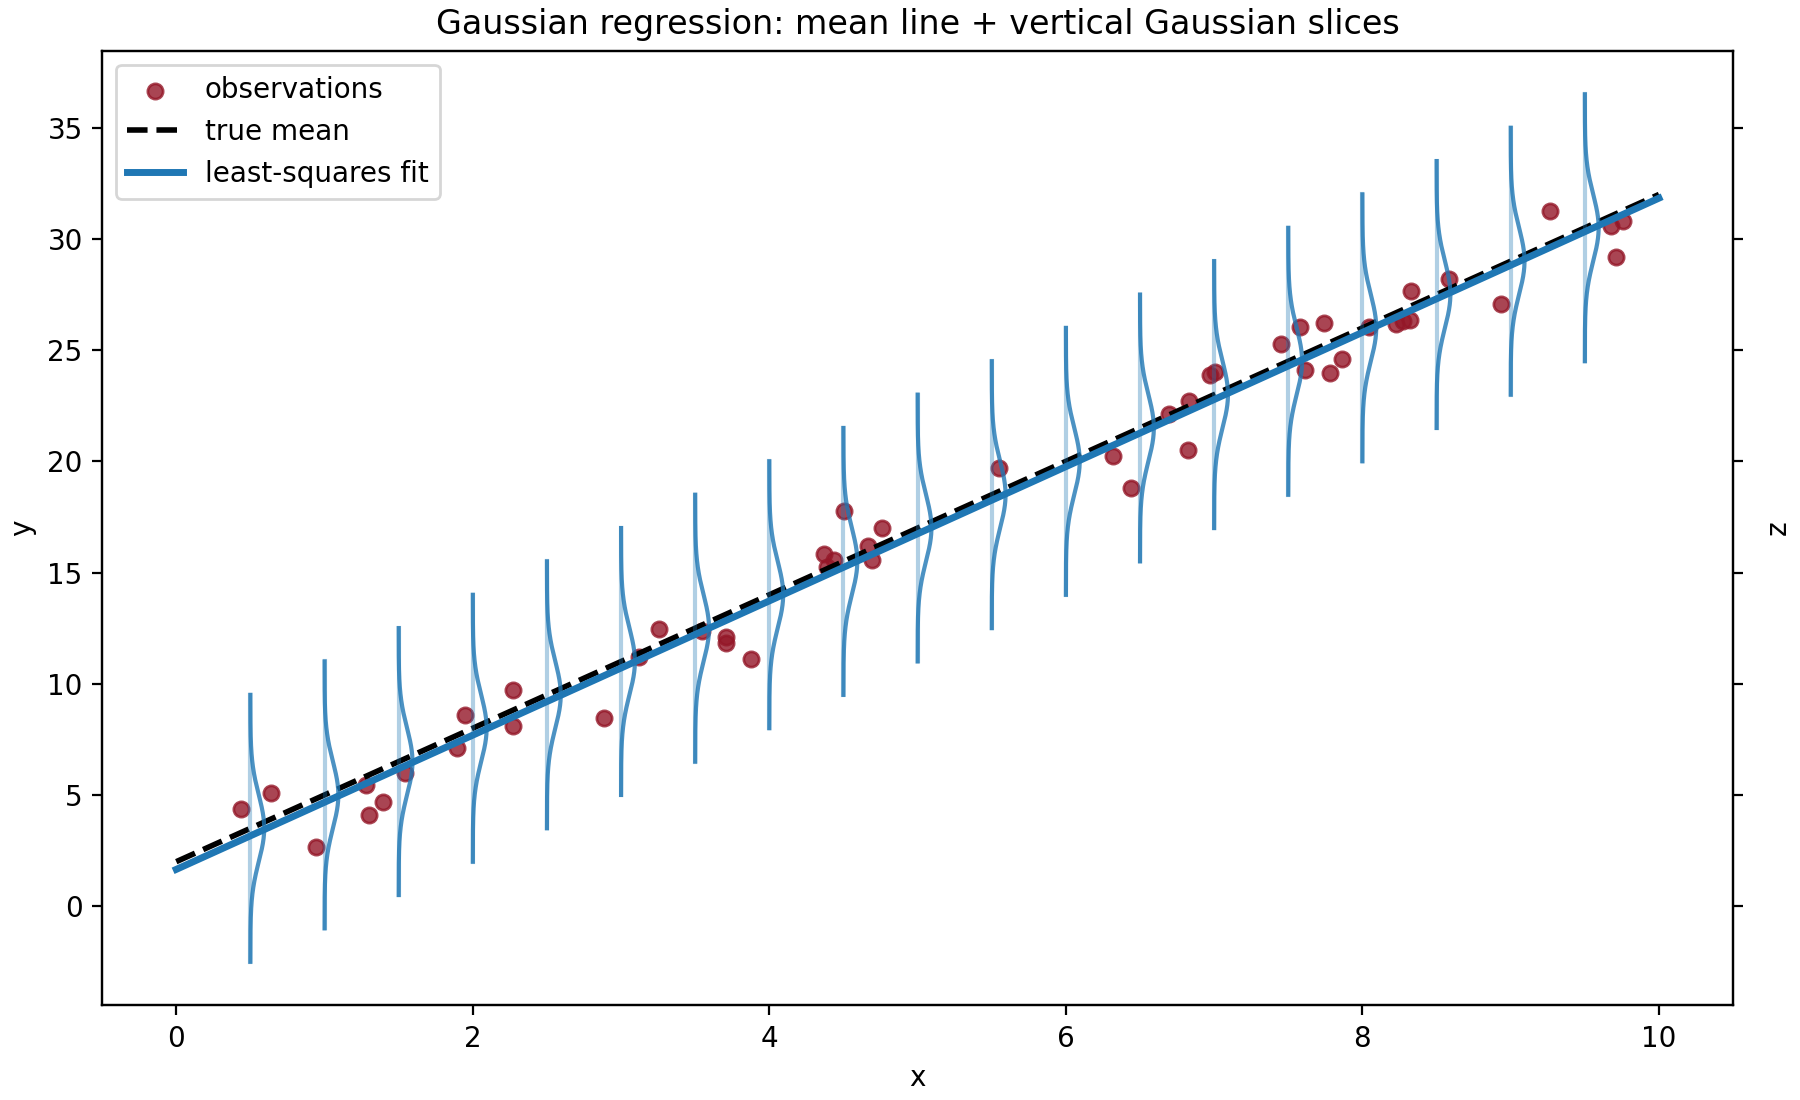
\includegraphics[width=0.8\textwidth]{../09_gaussian_regression/outputs/gaussian_regression.png}

\vspace{0.5em}
\small At each $x$, the model predicts a Gaussian over $y$ with mean $\mu(x) = mx + b$ and fixed noise scale $\sigma$
\note{Let's look at this figure carefully. The scatter points are noisy observations. The vertical Gaussian curves show the conditional distribution at selected x values. All the curves have the same width (constant sigma), but their centers follow the regression line. The true line (dashed) and fitted line (solid) are nearly identical because we have enough data.}
\end{frame}

\begin{frame}[c]{From likelihood to least squares}
\textbf{Given data:} $(x_1, y_1), (x_2, y_2), \ldots, (x_n, y_n)$

\vspace{0.5em}
\textbf{Model:} $Y_i \mid x_i \sim \mathcal{N}(mx_i + b, \sigma^2)$

\vspace{0.5em}
\textbf{Start with the likelihood:}
\[
\mathcal{L}(m, b) = \prod_{i=1}^n p(y_i \mid x_i; m, b, \sigma^2)
\]

\pause
\vspace{0.5em}

\textbf{Expand using the Gaussian formula:}
\[
\mathcal{L}(m, b) = \prod_{i=1}^n \frac{1}{\sqrt{2\pi\sigma^2}} \exp\left(-\frac{[y_i - (mx_i + b)]^2}{2\sigma^2}\right)
\]

\vspace{0.5em}
\textbf{Goal:} Find $m$ and $b$ that maximize this.
\note{We're setting up the same likelihood approach we used for the mean and variance, but now the parameters are m and b instead of mu. The key: each observed yi comes from a Gaussian centered at mxi + b.

[click]

The likelihood is the product of these Gaussian densities because observations are independent. Sigma is treated as a known constant here---we're only optimizing for m and b.}
\end{frame}

\begin{frame}[c]{Derivation: Take the log}
\textbf{Log-likelihood:}
\[
\log \mathcal{L}(m, b) = \sum_{i=1}^n \left[-\frac{1}{2}\log(2\pi\sigma^2) - \frac{[y_i - (mx_i + b)]^2}{2\sigma^2}\right]
\]

\pause
\vspace{0.5em}

\textbf{Drop constants that don't depend on $m$ or $b$:}
\[
\log \mathcal{L}(m, b) \propto -\frac{1}{2\sigma^2} \sum_{i=1}^n [y_i - (mx_i + b)]^2
\]

\pause
\vspace{0.5em}

\textbf{Maximizing this is equivalent to minimizing:}
\[
\sum_{i=1}^n [y_i - (mx_i + b)]^2
\]

\vspace{0.5em}
This is the \textbf{sum of squared residuals} --- exactly the least squares objective!
\note{Notice how the log converts the product to a sum. The constant term log(2pi*sigma²) doesn't contain m or b, so it drops out when we maximize.

[click]

The 1/(2sigma²) factor is positive, so maximizing the negative sum is the same as minimizing the positive sum.

[click]

The squared term [yi - (mxi + b)]² is the residual---the difference between observed yi and predicted mxi + b. This is exactly the least squares objective!}
\end{frame}

\begin{frame}[c]{The equivalence}
\textbf{Result:}
\[
\arg\max_{m,b} \mathcal{L}(m, b) = \arg\min_{m,b} \sum_{i=1}^n [y_i - (mx_i + b)]^2
\]

\vspace{1em}
\textbf{Maximum likelihood estimation} for Gaussian-distributed errors gives exactly the same $m$ and $b$ as \textbf{ordinary least squares}.

\vspace{1em}
\textbf{Finding $m$ and $b$:} Take partial derivatives with respect to $m$ and $b$, set to zero, and solve the resulting linear system. This is a classical linear algebra exercise.
\note{Squared error is not arbitrary---it emerges naturally from the Gaussian assumption. If you use least squares, you're implicitly assuming Gaussian noise. Many people who learned least squares in earlier courses don't realize this connection. The actual solution involves solving a 2×2 linear system (the normal equations), which you've likely seen in a linear algebra course. We don't need to rederive it here. This connection is bidirectional: if the noise is not Gaussian (e.g., heavy-tailed or skewed), least squares can perform poorly. What loss function would correspond to a Laplace distribution? Absolute error, not squared error. This foreshadows robust regression.}
\end{frame}

\begin{frame}[fragile]{Live demo}
\textbf{Demo 1:} Transform standard-normal samples
\begin{lstlisting}[language=bash]
cd mathematical_foundations/08_normal
conda run -n cse434 python3 08_normal_randn.py
\end{lstlisting}

\vspace{0.5em}
\textbf{Demo 2:} Central Limit Theorem — sample means are approximately normal
\begin{lstlisting}[language=bash]
cd mathematical_foundations/08_normal
conda run -n cse434 python3 08_normal_clt_demo.py
\end{lstlisting}

\vspace{0.5em}
\textbf{Demo 3:} Generate noisy linear data and fit by least squares
\begin{lstlisting}[language=bash]
cd mathematical_foundations/09_gaussian_regression
conda run -n cse434 python3 09_gaussian_regression.py
\end{lstlisting}

\vspace{0.5em}
All demos show the probabilistic ideas we just derived.
\note{I'll run the first demo and show you the shift and scale transformation in the code. The CLT demo shows that sample means are approximately normal and that variance decreases as 1/n — notice how this matches the sqrt(n) factor we discussed. For the regression demo, look at the vertical Gaussian slices in the plot---these visualize the conditional distribution Y given x. Can you identify the parameters m, b, and sigma from the printed output?}
\end{frame}

\begin{frame}[c]{Coming up next}
\textbf{Multivariate normal distributions:}
\begin{itemize}
    \item How continuous variables change together
    \item Covariance geometry
    \item Pixel correlations in images
    \item Latent-space structure in generative models
\end{itemize}

\vspace{1em}
\textbf{Further reading:}
\begin{itemize}
    \item PRML (Bishop): Sections 1.2.4, 1.2.5, and 2.3
    \item 3Blue1Brown: Central Limit Theorem
    \item 3Blue1Brown: Gaussian + Gaussian = Gaussian
    \item StatQuest: The Normal Distribution
\end{itemize}
\note{Next time we'll look at multivariate normal distributions. Today we modeled one variable at a time. Next time, we'll model multiple variables jointly and see how the covariance matrix encodes their relationships. The 3Blue1Brown videos are excellent visual supplements. Bishop's PRML is the canonical reference for the math.}
\end{frame}

\end{document}
